% !TEX root = ../main.tex

\label{appendix}

\begin{proof}[Proof that the determinant of the rotation matrix in two dimensions equals one \eqref{eq:constraint_det}\\]$\,$\\
	Let $\alpha \in [-\pi, \pi]$ be an arbitrary rotation angle. Then we have
	\begin{equation}
		\label{proof:det_one}
		\begin{aligned}
		 \det (R_{2D}(\alpha)) &= \det \begin{pmatrix} \cos(\alpha) & -\sin(\alpha) \\\sin(\alpha) & \cos(\alpha) \end{pmatrix} \\
		&= \cos(\alpha)\cos(\alpha) - \sin(\alpha)(- \sin(\alpha))\\
		&= \cos(\alpha)^2 + \sin(\alpha)^2\\
		&= 1
		\end{aligned}
	\end{equation}
\end{proof}

\begin{proof}[Proof that the determinant of the rotation matrix in three dimensions equals one \eqref{eq:constraint_det}\\]$\,$\\
	Let $\alpha \in [-\pi, \pi]^2$ be an arbitrary rotation angle. Then we have
	\begin{equation}
	\label{proof:det_one_dim3}
	\begin{aligned}
	\det (R_{3D}(x, \vec{\alpha})) &= \det(R_{y}(\alpha_2) R_{z}(\alpha_1)) \\
	&= \det \left( \begin{pmatrix} \cos(\alpha_2) & -\sin(\alpha_2) & 0\\\sin(\alpha_2) & \cos(\alpha_2) & 0\\ 0 & 0 & 1\end{pmatrix} \begin{pmatrix} \cos(\alpha_1) & 0 & -\sin(\alpha_1)\\ 0 & 1 & 0\\\sin(\alpha_1) & 0 & \cos(\alpha_1)\end{pmatrix} \right)\\
	&= \det \begin{pmatrix} \cos(\alpha_2) & -\sin(\alpha_2) & 0\\\sin(\alpha_2) & \cos(\alpha_2) & 0\\ 0 & 0 & 1\end{pmatrix} \cdot \det \begin{pmatrix} \cos(\alpha_1) & 0 & -\sin(\alpha_1)\\ 0 & 1 & 0\\\sin(\alpha_1) & 0 & \cos(\alpha_1)\end{pmatrix}\\
	&= (\cos(\alpha_2)^2 + \sin(\alpha_2)^2) \cdot (\cos(\alpha_1)^2 + \sin(\alpha_1)^2)\\
	&= 1
	\end{aligned}
	\end{equation}
\end{proof}

\begin{proof}[Proof for the norm preservation by the rotation in two dimensions \eqref{eq:constraint_norm}\\]$\,$\\
	Let $p = \begin{pmatrix}x \\y \\\end{pmatrix}$ be any input vector with $x, y \in \mathbb{R}$ and $\alpha \in [-\pi, \pi]$ an arbitrary rotation angle. Since $||\cdot|| \geq 0$, it is sufficient to show that $||rot_{2D}(p, \vec{\alpha})||_2^2 = ||p||_2^2$.
	\begin{equation}
	\label{proof:norm_preservation}
	\begin{aligned}
	||rot_{2D}(p, \alpha)||_2 &= \left\Vert \begin{pmatrix} \cos(\alpha) & -\sin(\alpha) \\\sin(\alpha) & \cos(\alpha) \end{pmatrix} \begin{pmatrix}x \\y \\\end{pmatrix} \right\Vert_2^2 \\
	&= (\cos(\alpha)x - \sin(\alpha)y)^2 + (\sin(\alpha)x + \cos(\alpha)y)^2\\
	&= \cos(\alpha)^2x^2 -2\cos(\alpha)x\sin(\alpha)y \sin(\alpha)^2y^2 + \sin(\alpha)^2y^2\\ &\,\,\,\,\,\,\,\,\,+ \sin(\alpha)^2x^2 + 2\sin(\alpha)x\cos(\alpha)y + \cos(\alpha)^2y^2\\
	&= (\cos(\alpha)^2 + \sin(\alpha)^2)x^2 + (\sin(\alpha)^2 + \cos(\alpha)^2)y^2\\
	&= x^2 + y^2\\
	&= ||p||_2^2
	\end{aligned}
	\end{equation}
\end{proof}

\begin{proof}[Proof for the norm preservation by the rotation in three dimensions \eqref{eq:constraint_norm}\\]$\,$\\
	Let $p = \begin{pmatrix}x \\y \\z \\\end{pmatrix}$ be any input vector with $x, y, z \in \mathbb{R}$ and $\alpha \in [-\pi, \pi]^2$ an arbitrary rotation angle. Since $||\cdot|| \geq 0$, it is sufficient to show that $||rot_{3D}(p, \vec{\alpha})||_2^2 = ||p||_2^2$.
	\begin{equation}
	\label{proof:norm_preservation_dim3}
	\begin{aligned}
	||rot_{3D}(p, \vec{\alpha})||_2^2 &= \left\Vert R_{y}(\alpha_2) R_{z}(\alpha_1) p \right\Vert_2^2 \\
	&= \left\Vert \begin{pmatrix} \cos(\alpha_2) & -\sin(\alpha_2) & 0\\\sin(\alpha_2) & \cos(\alpha_2) & 0\\ 0 & 0 & 1\end{pmatrix} \begin{pmatrix} \cos(\alpha_1) & 0 & -\sin(\alpha_1)\\ 0 & 1 & 0\\\sin(\alpha_1) & 0 & \cos(\alpha_1)\end{pmatrix} \begin{pmatrix}x \\y \\z \\\end{pmatrix} \right\Vert_2^2 \\
	&= \left\Vert \begin{pmatrix} \cos(\alpha_2) & -\sin(\alpha_2) & 0\\\sin(\alpha_2) & \cos(\alpha_2) & 0\\ 0 & 0 & 1\end{pmatrix} \begin{pmatrix}\cos(\alpha_1)x - \sin(\alpha_1)z \\y \\\sin(\alpha_1)x + \cos(\alpha_1)z \\\end{pmatrix} \right\Vert_2^2 \\
	&= \left\Vert \begin{pmatrix}\cos(\alpha_2)(\cos(\alpha_1)x - \sin(\alpha_1)z) - \sin(\alpha_2)y \\
	\sin(\alpha_2)(\cos(\alpha_1)x - \sin(\alpha_1)z) + \cos(\alpha_2)y \\
	\sin(\alpha_1)x + \cos(\alpha_1)z \\\end{pmatrix} \right\Vert_2^2 \\
	&= (\cos(\alpha_2)^2 + \sin(\alpha_2)^2)(\cos(\alpha_1)x - \sin(\alpha_1)z)^2 + \sin(\alpha_2)^2y^2 + \cos(\alpha_2)^2y^2 \\ 
	&\,\,\,\,\,\,\,\,\,+ \sin(\alpha_1)^2x^2 + 2\sin(\alpha_1)x\cos(\alpha_1)z + \cos(\alpha_1)^2z^2\\
	&= \cos(\alpha_1)^2x^2 + \sin(\alpha_1)^2z^2 + y^2 + \sin(\alpha_1)^2x^2 + \cos(\alpha_1)^2z^2\\
	&= x^2 + y^2 + z^2\\
	&= ||p||_2^2
	\end{aligned}
	\end{equation}
\end{proof}

\begin{figure}[H]
	\centering
	\begin{subfigure}{.5\textwidth}
		\centering
		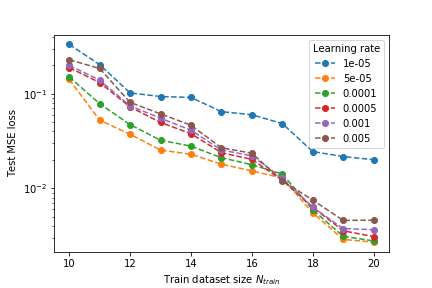
\includegraphics[width=\linewidth]{lr_dim2_m3}
		\caption{2 dimensions}
	\end{subfigure}%
	\begin{subfigure}{.5\textwidth}
		\centering
		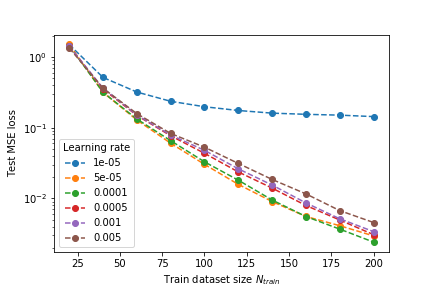
\includegraphics[width=\linewidth]{lr_dim3_m3}
		\caption{3 dimensions}
	\end{subfigure}
	\caption{Comparison of learning rates for Model 3}
	\label{fig:comp_lr_m3}
\end{figure}

\begin{figure}[H]
	\centering
	\begin{subfigure}{.5\textwidth}
		\centering
		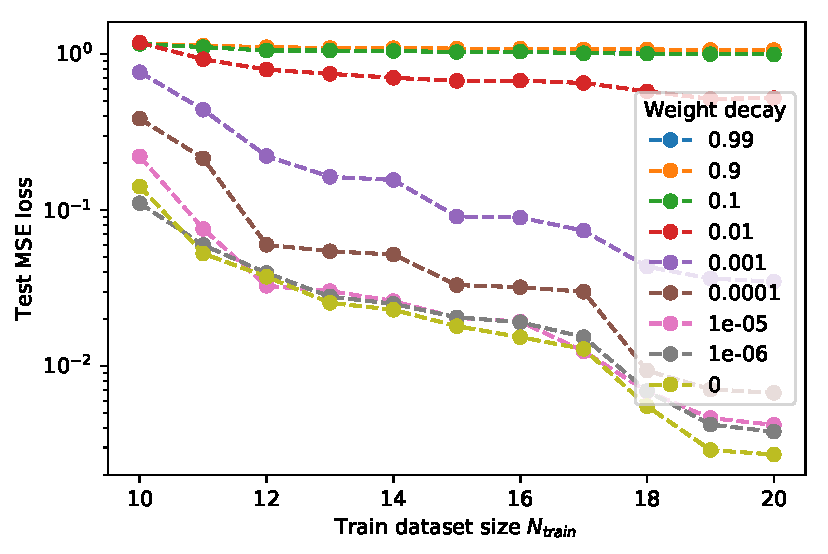
\includegraphics[width=\linewidth]{reg_weights}
		\caption{2 dimensions}
	\end{subfigure}%
	\begin{subfigure}{.5\textwidth}
		\centering
		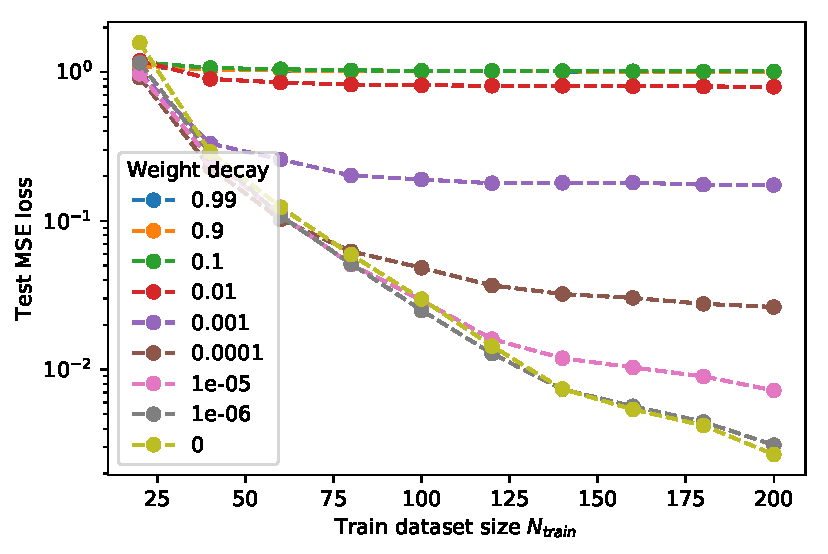
\includegraphics[width=\linewidth]{reg_weights_dim3}
		\caption{3 dimensions}
	\end{subfigure}
	\caption{L2-Regularisation weights on Model 3}
	\label{fig:reg_weights}
\end{figure}


\begin{figure}[H]
	\centering
	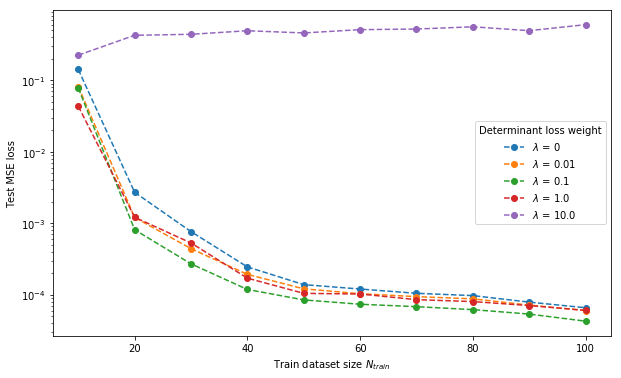
\includegraphics[width=0.8\linewidth]{pnlty_det_large}
	\caption{Performance of Model 3 when applying the Fixed Penalty Method with different weights $\lambda$ for $\mathcal{L}_{DET}$ in 2 dimensions.}
	\label{fig:pnlty_det_large}
\end{figure}

\begin{figure}[H]
	\centering
	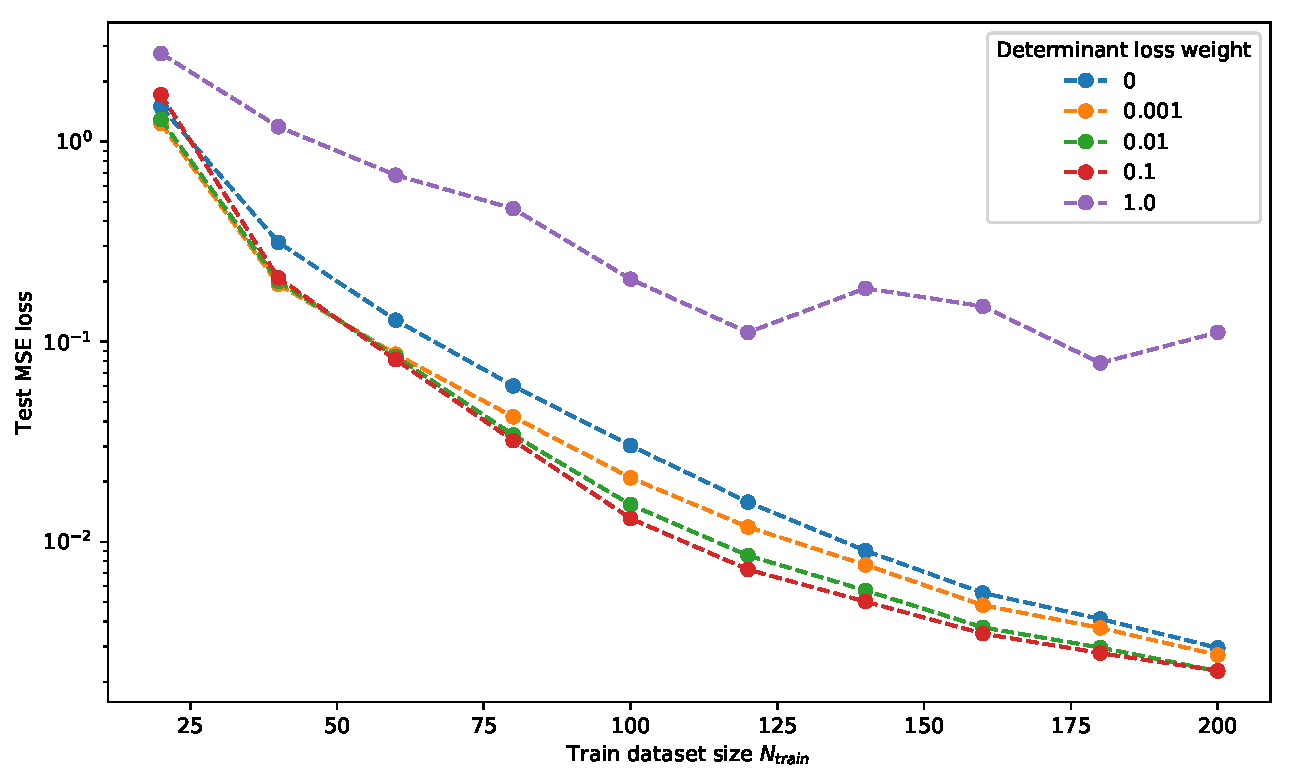
\includegraphics[width=0.8\linewidth]{pnlty_det_dim3}
	\caption{Performance of Model 3 when applying the Fixed Penalty Method with different weights $\lambda$ for $\mathcal{L}_{DET}$ in 3 dimensions.}
	\label{fig:pnlty_det_dim3}
\end{figure}

\begin{figure}[H]
	\centering
	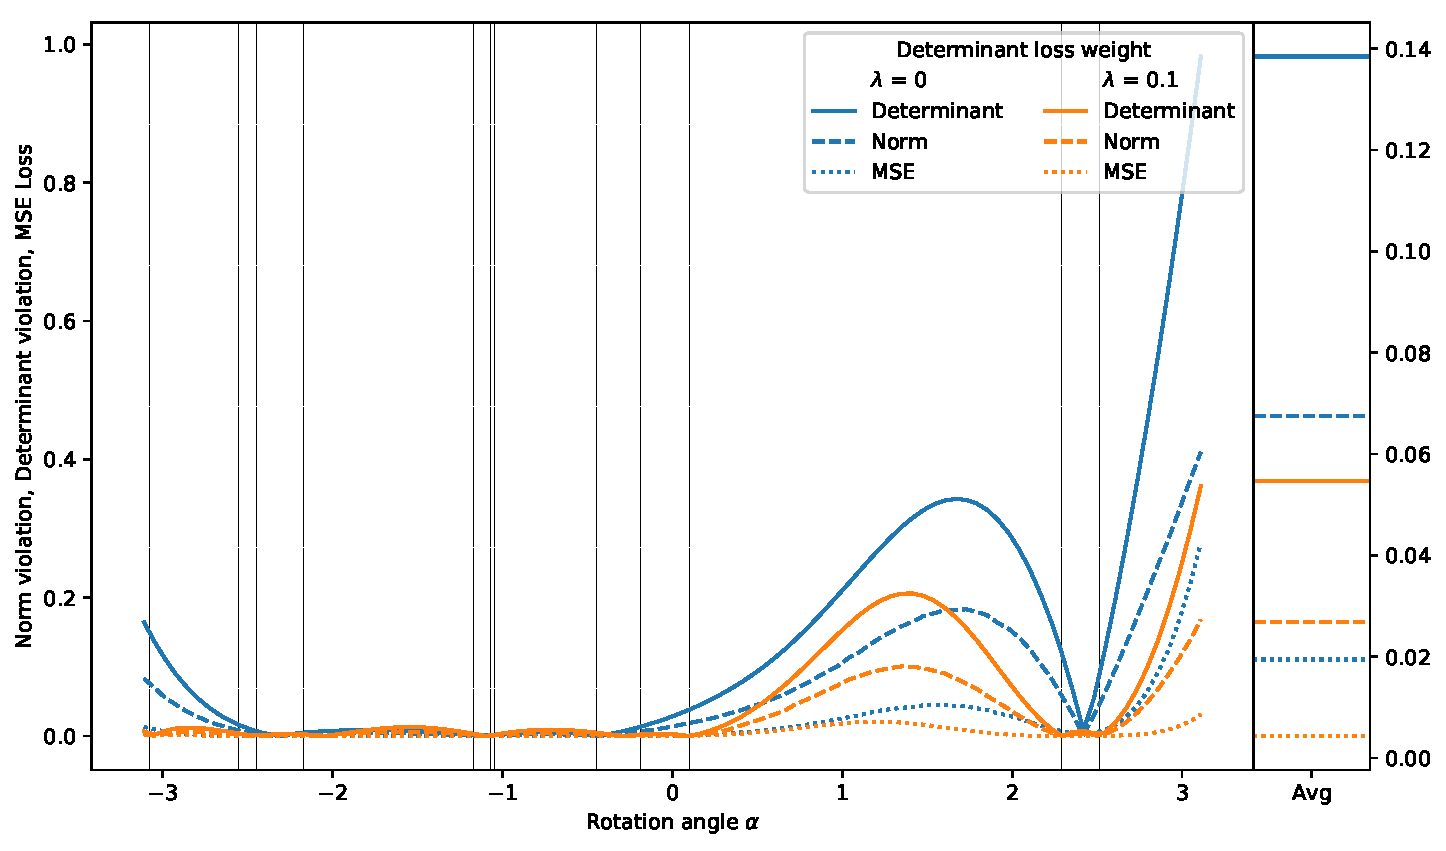
\includegraphics[width=0.8\linewidth]{pnlty_det_analysis_model2}
	\caption{Determinant and norm violations of predictions for $N_{train} = 12$ using Model 2. Gray vertical lines represent the angles of the training points.}
	\label{fig:pnlty_det_analysis_model2}
\end{figure}

\begin{figure}[H]
\centering
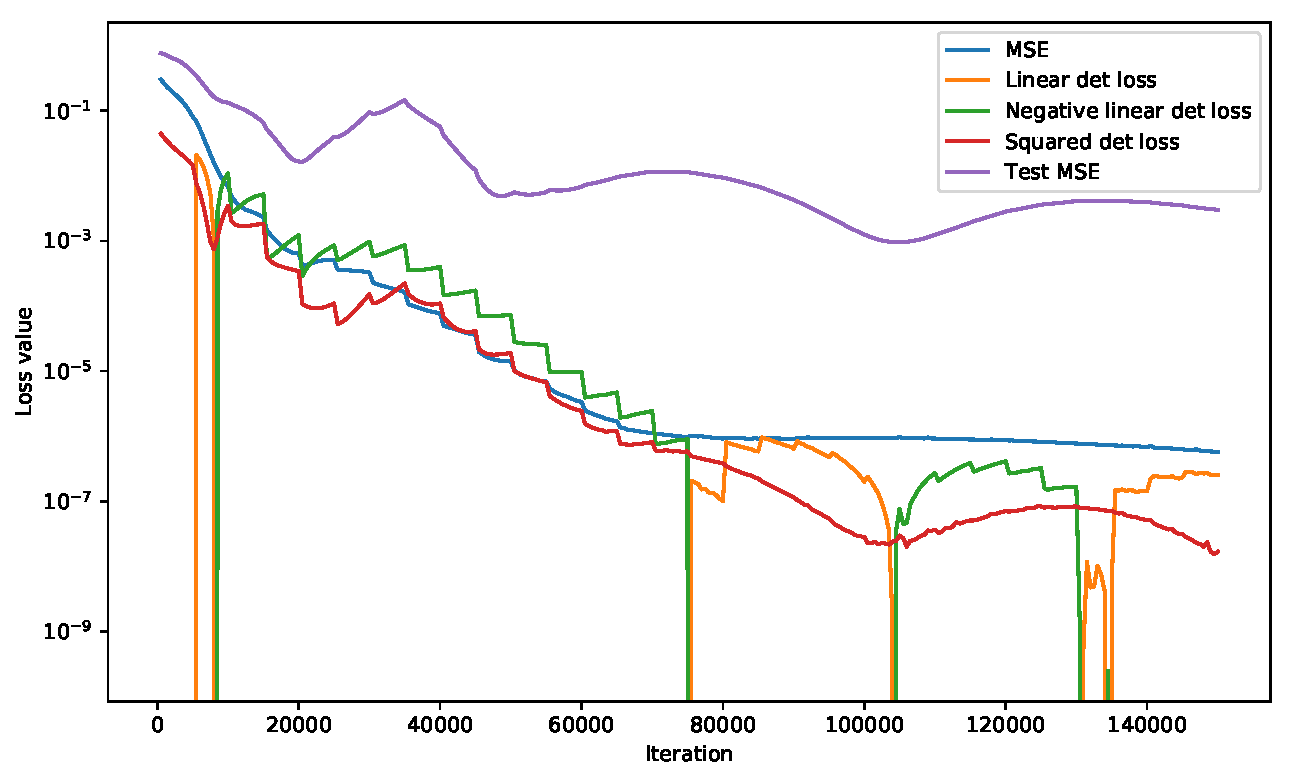
\includegraphics[width=0.7\linewidth]{alm_fixed_training}
\caption{Loss values during training of the fixed ALM in 2D for $N_{train} = 12$ and a single random seed.}
\label{fig:alm_fixed_training}
\end{figure}

\begin{table}[H]
\centering
\resizebox{\columnwidth}{!}{%
\begin{tabular}{lrrrrrrrr}
	\midrule
	{} &  count &      mean &       std &       min &       25\% &       50\% &       75\% &       max \\ \midrule
	Original ($\lambda = 0$)         &   10.0 &  0.083873 &  0.084808 &  0.017509 &  0.025126 &  0.051635 &  0.102614 &  0.258126 \\ \midrule
	Penalty method ($\lambda = 0.1$) &   10.0 &  0.061773 &  0.089446 &  0.002449 &  0.006697 &  0.018631 &  0.095302 &  0.280234 \\ \midrule
	ALM fixed                        &   10.0 &  0.036335 &  0.041466 &  0.001796 &  0.007078 &  0.014448 &  0.054447 &  0.119299 \\ \midrule
	ALM dynamic                      &   10.0 &  0.028551 &  0.026700 &  0.005898 &  0.009325 &  0.017179 &  0.041241 &  0.079159 \\ \midrule
\end{tabular}
}
\caption{Test MSE Loss statistics for 10 random training sets and $N_{train} = 10$}
\label{table_stats_10}
\end{table}

\begin{table}[H]
	\centering
	\resizebox{\columnwidth}{!}{%
		\begin{tabular}{lrrrrrrrr}
			{} &  count &      mean &       std &       min &       25\% &       50\% &       75\% &       max \\ \midrule
			Original ($\lambda = 0$)         &   10.0 &  0.012718 &  0.009706 &  0.000652 &  0.006690 &  0.010347 &  0.014473 &  0.032356 \\ \midrule
			Penalty method ($\lambda = 0.1$) &   10.0 &  0.002330 &  0.001577 &  0.000174 &  0.001137 &  0.002370 &  0.003468 &  0.004632 \\ \midrule
			ALM fixed                        &   10.0 &  0.001832 &  0.001621 &  0.000128 &  0.000656 &  0.001172 &  0.002869 &  0.004497 \\ \midrule
			ALM dynamic                      &   10.0 &  0.001889 &  0.001693 &  0.000094 &  0.000804 &  0.001271 &  0.002364 &  0.005209 \\ \midrule
		\end{tabular}
	}
	\caption{Test MSE Loss statistics for 10 random training sets and $N_{train} = 15$}
	\label{table_stats_15}
\end{table}

\begin{table}[H]
	\centering
	\resizebox{\columnwidth}{!}{%
		\begin{tabular}{lrrrrrrrr}
			{} &  count &      mean &       std &       min &       25\% &       50\% &       75\% &       max \\ \midrule
			Original ($\lambda = 0$)         &   10.0 &  0.002534 &  0.002381 &  0.000539 &  0.000931 &  0.001674 &  0.003141 &  0.007491 \\ \midrule
			Penalty method ($\lambda = 0.1$) &   10.0 &  0.000703 &  0.000487 &  0.000154 &  0.000260 &  0.000686 &  0.000999 &  0.001665 \\ \midrule
			ALM fixed                        &   10.0 &  0.000394 &  0.000422 &  0.000072 &  0.000140 &  0.000174 &  0.000511 &  0.001419 \\ \midrule
			ALM dynamic                      &   10.0 &  0.000349 &  0.000332 &  0.000016 &  0.000072 &  0.000211 &  0.000564 &  0.000922 \\ \midrule
		\end{tabular}
	}
	\caption{Test MSE Loss statistics for 10 random training sets and $N_{train} = 20$}
	\label{table_stats_20}
\end{table}


\begin{figure}[H]
	\centering
	\begin{subfigure}{.5\textwidth}
		\centering
		\includegraphics[width=\linewidth]{lag_mu}
		\caption{Physical loss weight $\mu$}
	\end{subfigure}%
	\begin{subfigure}{.5\textwidth}
		\centering
		\includegraphics[width=\linewidth]{lag_est}
		\caption{Lagrangian multiplier estimates $\lambda$}
	\end{subfigure}
	\caption{Values for the physical loss weight $\mu$ and the Lagrangian multiplier estimates $\lambda$ when training using the dynamic ALM with $N_{train} = 12$.}
	\label{fig:mu_lambda_alm_dyn}
\end{figure}


\begin{figure}[H]
	\centering
	\begin{subfigure}{.5\textwidth}
		\centering
		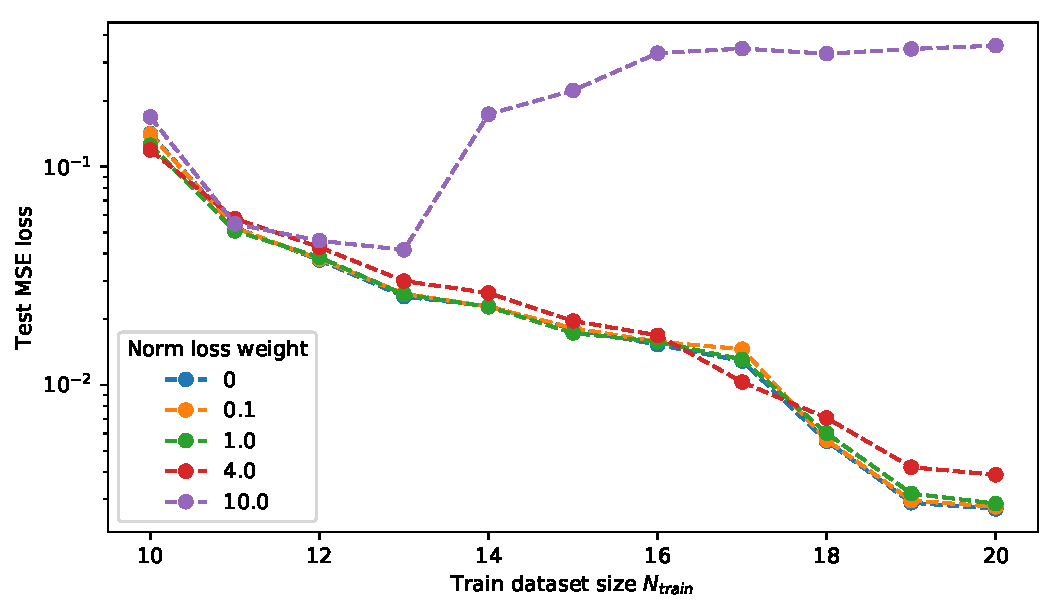
\includegraphics[width=\linewidth]{pnlty_norm}
		\caption{2 dimensions}
	\end{subfigure}%
	\begin{subfigure}{.5\textwidth}
		\centering
		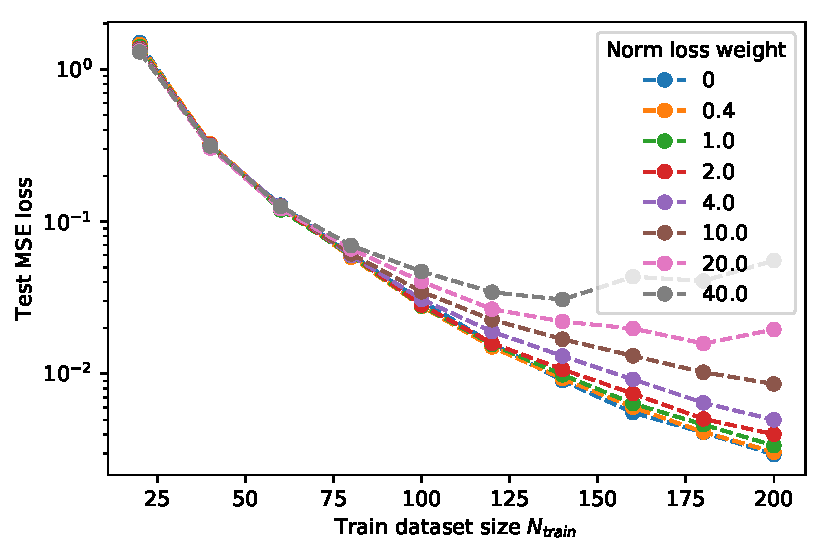
\includegraphics[width=\linewidth]{pnlty_norm_3}
		\caption{3 dimensions}
	\end{subfigure}
	\caption{Penalty Method on the Norm constraint}
	\label{fig:pnlny_norm}
\end{figure}


\begin{figure}[H]
	\centering
	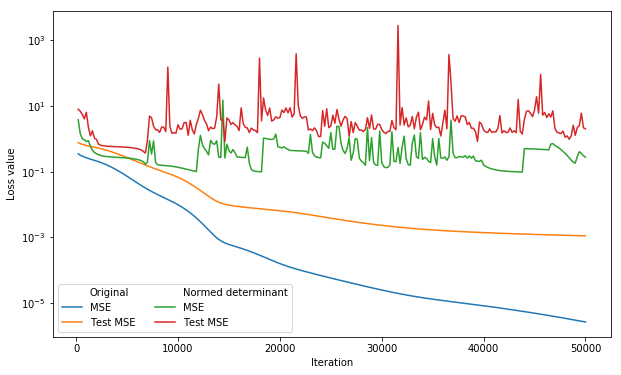
\includegraphics[width=0.7\linewidth]{normed_det_example}
	\caption{Training for 2 dimensions and $N_{train} = 20$ using the original training and the Physical projection on the determinant with the same training dataset.}
	\label{fig:normed_det_example}
\end{figure}

\begin{figure}[H]
	\centering
	\begin{subfigure}{.5\textwidth}
		\centering
		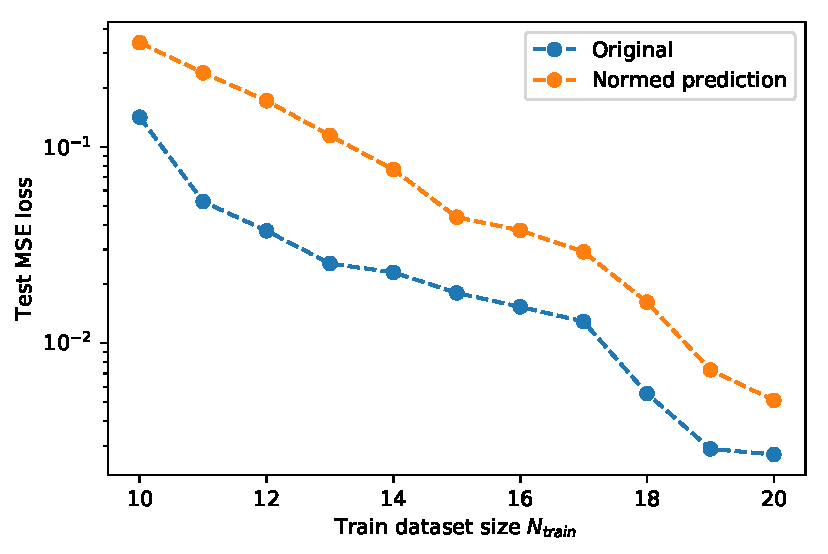
\includegraphics[width=\linewidth]{normed_pred}
		\caption{2 dimensions}
	\end{subfigure}%
	\begin{subfigure}{.5\textwidth}
		\centering
		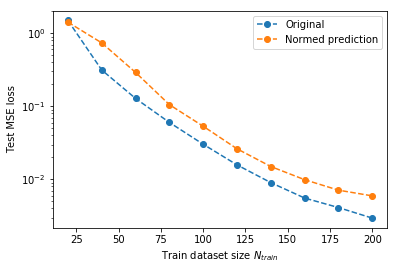
\includegraphics[width=\linewidth]{normed_pred_3}
		\caption{3 dimensions}
	\end{subfigure}
	\caption{Physical projection on the norm of the prediction}
	\label{fig:normed_pred}
\end{figure}

\begin{figure}[H]
	\centering
	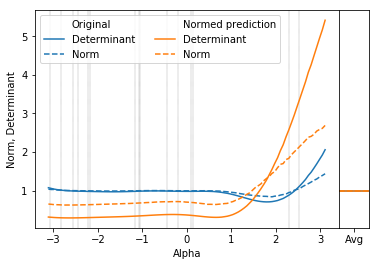
\includegraphics[width=0.7\linewidth]{normed_pred_example}
	\caption{Analysis of the predictions of a model trained using Physical Projection on the norm compared to the original model. All determinants and norms are scaled such that their mean is equal to one.}
	\label{fig:normed_pred_example}
\end{figure}


\clearpage
